% !TeX program = xelatex
% Overleaf: Menu -> Compiler -> XeLaTeX (not pdfLaTeX)
\documentclass[aspectratio=169,11pt]{beamer}
\usepackage[UTF8,fontset=fandol]{ctex}
\usepackage{amsmath,amssymb,bm,booktabs,graphicx,mathtools,array}
\usepackage{tikz}
\usetikzlibrary{arrows.meta,positioning,shapes.geometric}
\usepackage{hyperref}
\definecolor{navy}{HTML}{17324D}
\definecolor{teal}{HTML}{157A82}
\definecolor{light}{HTML}{EFF5F6}
\definecolor{warn}{HTML}{A85D20}
\setbeamercolor{normal text}{fg=navy,bg=white}
\setbeamercolor{structure}{fg=teal}
\setbeamercolor{frametitle}{fg=navy,bg=light}
\setbeamercolor{title}{fg=navy}
\setbeamercolor{block title}{bg=teal!15,fg=navy}
\setbeamercolor{block body}{bg=teal!5,fg=navy}
\setbeamertemplate{navigation symbols}{}
\setbeamertemplate{footline}{\hfill\scriptsize PrimitiveCAD 论文解读\quad\insertframenumber/\inserttotalframenumber\hspace{1em}\vspace{0.8em}}
\setbeamertemplate{itemize item}[circle]
\setbeamertemplate{itemize subitem}[triangle]
\setbeamersize{text margin left=0.65cm,text margin right=0.65cm}
\newcommand{\source}[1]{\par\vspace{0.25em}{\tiny\color{gray}来源：#1}}
\newcommand{\tagpaper}{\textcolor{teal}{\bfseries [论文]}}
\newcommand{\taginfer}{\textcolor{warn}{\bfseries [分析]}}
\newcommand{\tagunknown}{\textcolor{warn}{\bfseries [待验证]}}
\newcommand{\tight}{\setlength{\itemsep}{0.24em}}
\title{PrimitiveCAD：结构感知的 Point-to-CAD 重建}
\subtitle{从研究动机、完整 Pipeline 到数学推导、实验与 Follow-up}
\author{论文精读 / Research Presentation}
\date{Gao et al. \quad ACM Multimedia 2026 \quad arXiv:2610.08698v1}
\begin{document}

\begin{frame}[plain]
\titlepage
\end{frame}

\begin{frame}{阅读路线与证据规则}
\begin{columns}[T]
\column{0.53\textwidth}
\begin{enumerate}\tight
\item 任务是什么，为什么重要？
\item 已有方法的失败模式
\item 从已有知识重建研究直觉
\item 三阶段算法与关键公式
\item 消融、结果和 claim 的边界
\item 脆弱假设、最小复现、反例
\item 一个非增量的后续研究方向
\end{enumerate}
\column{0.45\textwidth}
\begin{block}{证据等级}
\tagpaper\ 原文清楚陈述/实验报告\\[0.4em]
\textcolor{teal}{\bfseries [文献]}\ 已有研究支持\\[0.4em]
\taginfer\ 基于证据的分析\\[0.4em]
\tagunknown\ 尚需额外实验核实
\end{block}
\end{columns}
\end{frame}

\section{任务与背景}
\begin{frame}{1. 研究问题：由点云恢复可执行 CAD 程序}
\begin{columns}[c]
\column{0.5\textwidth}
\begin{center}
\includegraphics[width=\linewidth]{figures/paper_teaser.png}\end{center}
\column{0.49\textwidth}
\begin{block}{输入与输出}
输入：零件表面点云 $P=\{\bm p_i\}_{i=1}^N$, $\bm p_i\in\mathbb R^3$\\[0.3em]
输出：可执行的 \texttt{CadQuery/Python} 程序 $C$\\[0.3em]
执行：$C\longrightarrow M(C)$，得到参数化 CAD 实体
\end{block}
\begin{itemize}\tight
\item 要恢复尺寸、孔、凸台等局部特征
\item 输出程序需能运行并生成有效实体
\item 外形重建与\alert{原始设计历史恢复}不是同一任务
\end{itemize}
\end{columns}
\source{原论文 Figure 1，p.1；§3.1，p.3}
\end{frame}

\begin{frame}{为何输出 CAD 代码，而不仅是 Mesh？}
\begin{table}\centering\small
\begin{tabular}{lll}\toprule
表示 & 主要承载信息 & 参数修改能力\\\midrule
点云 & 离散表面坐标 & 无直接建模语义\\
Triangle Mesh & 三角片构成的表面 & 一般需额外几何编辑\\
B-Rep & 几何曲面、边和拓扑 & 依赖 CAD 编辑机制\\
参数化 CAD 程序 & 构造操作及参数 & 能重新执行并改变参数\\\bottomrule
\end{tabular}
\end{table}
\begin{block}{工程价值 \taginfer}
扫描逆向工程、零件再设计、CAD 自动化；但论文尚未直接评估\textbf{制造公差、装配约束、参数化编辑成功率}。
\end{block}
\end{frame}

\begin{frame}{2. 先前工作解决了什么？}
\small
\begin{table}\centering
\begin{tabular}{p{2.5cm}p{4.6cm}p{5.2cm}}\toprule
路线 & 核心进展 & 仍存在的缺口\\\midrule
DeepCAD (2021) & 将草图/拉伸建模为离散操作序列 & 有限的任务专用指令空间\\
Point2Cyl / TransCAD & 从点云推断几何原语或建模序列 & 受几何表示与操作模板限制\\
CAD-Recode (2025) & 生成可执行 CadQuery Python 程序 & 特定 CAD 结构监督不足\\
Cadrille (2025) & 多模态输入 + 执行反馈的 RL & 细粒度几何特征未显式对齐\\\bottomrule
\end{tabular}
\end{table}
\begin{block}{核心矛盾}
把 Point-to-CAD 视作通用的点云编码 + 下一个 Token 预测，会遗漏 CAD 特有的\textbf{几何实例、构造操作、边界特征}。
\end{block}
\source{原论文 §1–2；DeepCAD (ICCV 2021), CAD-Recode (ICCV 2025), Cadrille (2025)}
\end{frame}

\begin{frame}{典型失败模式：知道零件大概长什么样，仍会出错}
\begin{columns}[T]
\column{0.32\textwidth}
\begin{block}{输入感知失误}
多个圆柱面混成一个结构；小孔与实心凸台混淆。\\[0.5em]
\textbf{对应：}几何原语表征
\end{block}
\column{0.32\textwidth}
\begin{block}{代码结构失误}
漏掉一个圆/一次拉伸，或者产生多余操作。\\[0.5em]
\textbf{对应：}操作数量监督
\end{block}
\column{0.32\textwidth}
\begin{block}{评价反馈失误}
小孔漏掉后，主体仍占几乎全部体积；IoU 惩罚可能很弱。\\[0.5em]
\textbf{对应：}特征线奖励
\end{block}
\end{columns}
\vspace{1em}
\centering\large\bfseries 重要：三个失败模式发生在不同的学习环节。
\end{frame}

\begin{frame}{3. 重建作者可能的思路（分析，不是作者自述）}
\small
\begin{enumerate}\setlength{\itemsep}{0.52em}
\item \textbf{接受已有范式：} Point Cloud $\rightarrow$ Encoder $\rightarrow$ LLM $\rightarrow$ CAD Python。
\item \textbf{看失败样本：}混淆几何实例、遗漏操作、丢失小孔；并非单一问题。
\item \textbf{利用现成监督：}有 GT CAD 程序，就能推导几何 primitive 标签及操作统计。
\item \textbf{利用现成技术：}法向预测、实例分割、Hungarian 匹配、soft count、GRPO。
\item \textbf{把不同信号放在对应位置：}点级语义 $\rightarrow$ 程序级组成 $\rightarrow$ 实体级质量。
\end{enumerate}
\begin{block}{核心 Intuition}
\textbf{CAD 是几何上有结构、执行后有确定结果的程序。}监督应从单一 Token 粒度扩展到多个 CAD 结构粒度。
\end{block}
\end{frame}

\section{方法}
\begin{frame}{4. 方法全景：三个训练阶段}
\centering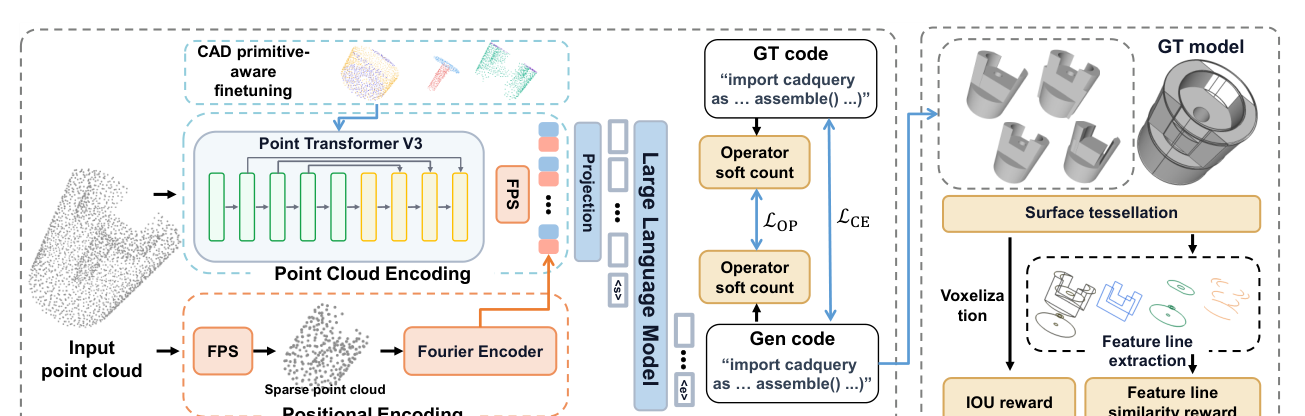
\includegraphics[width=0.98\linewidth,height=0.67\textheight,keepaspectratio]{figures/pipeline_original.png}
\vspace{0.15em}
\begin{columns}[T]
\column{0.32\textwidth}\centering\small\textbf{1. Primitive-aware PTv3}\\点级几何监督
\column{0.32\textwidth}\centering\small\textbf{2. SFT + Operation Alignment}\\程序级统计监督
\column{0.32\textwidth}\centering\small\textbf{3. GRPO + Feature Lines}\\实体执行反馈
\end{columns}
\source{原论文 Figure 2，p.3}
\end{frame}

\begin{frame}{5. 示例：一块三孔安装板如何被重建？}
\begin{columns}[T]
\column{0.48\textwidth}
\begin{block}{示意输入（自拟，不属于论文样本）}
\begin{itemize}\tight
\item 板尺寸：$80\times40\times10\,\mathrm{mm}$
\item 三个贯穿孔，直径 $8\,\mathrm{mm}$
\item 表面点云：$P\in\mathbb R^{1024\times3}$
\end{itemize}
\end{block}
\begin{block}{目标输出}
\texttt{box(80,40,10)}\\
\texttt{.faces(">Z").workplane()}\\
\texttt{.pushPoints([...]).hole(8)}
\end{block}
\column{0.48\textwidth}
\begin{block}{逐级处理}
1. PTv3 建模孔壁、平面、圆柱等结构\\[0.5em]
2. FPS 选 256 个点；输出 256 个几何 Embeddings\\[0.5em]
3. LLM 生成代码；SFT 约束关键操作统计\\[0.5em]
4. RL 执行代码，检查整体实体和圆形/直线边界
\end{block}
\end{columns}
\source{Pipeline 由 §3 重建；零件尺寸、具体代码均为讲解示例}
\end{frame}

\begin{frame}{Stage 1：PTv3 不是直接冻结使用}
\begin{columns}[T]
\column{0.5\textwidth}
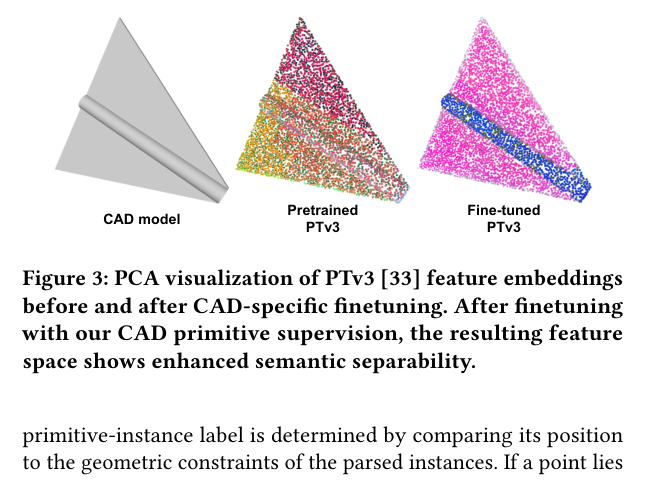
\includegraphics[width=\linewidth]{figures/ptv3_pca.png}
\column{0.5\textwidth}
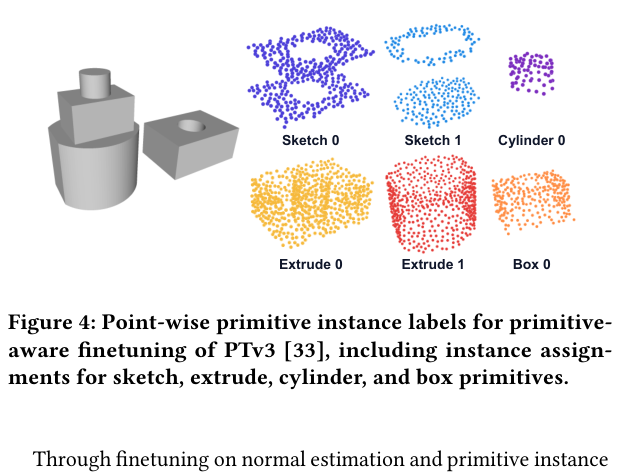
\includegraphics[width=\linewidth]{figures/primitive_labels.png}
\end{columns}
\begin{itemize}\tight
\item 在 PTv3 上添加两个头：$\hat{\bm n}_i\in\mathbb R^3$ 与 $\hat{\bm s}_i\in\mathbb R^{32}$。
\item 4 类实例：Sketch、Extrude、Cylinder、Box；每类最多 8 个实例槽位。
\item $32$ 指\textbf{实例槽位数}，不是 32 种几何 Primitive。
\end{itemize}
\source{原论文 Figures 3–4，p.4}
\end{frame}

\begin{frame}{Stage 1 数学：法向与无序实例监督}
\small
\begin{align*}
\mathcal L_{\mathrm{PT}}&=\mathcal L_n+\lambda_{\mathrm{PT}}\mathcal L_{\mathrm{seg}},\\
\mathcal L_n&=1-\frac{1}{N}\sum_{i=1}^{N}\left|\hat{\bm n}_i\cdot\bm n_i\right|,\\
\mathcal L_{\mathrm{seg}}&=1-\mathrm{RIoU}\bigl(\pi(\hat S),S\bigr),\\
\mathrm{RIoU}(X,Y)&=\frac{X^{\top}Y}{\lVert X\rVert_1+\lVert Y\rVert_1-X^{\top}Y}.
\end{align*}
\begin{itemize}\tight
\item 法向有符号歧义：$\bm n$ 与 $-\bm n$ 对应相同的无向表面方向。
\item 实例 ID 无确定顺序：通过 Hungarian Algorithm 寻找最优一对一排列 $\pi$。
\item 此处 RIoU 作用于 $[0,1]$ 的分割概率掩码；矩阵聚合细节在原文中被简写。
\end{itemize}
\source{原论文式 (2)–(5)，p.4；法向假设单位归一化}
\end{frame}

\begin{frame}{Stage 1 数学：空间位置如何进入 LLM？}
\small
\begin{align*}
F&=\mathrm{PTv3}(P)\in\mathbb R^{N\times64},\\
\phi(x)&=\left[x,\sin(\omega_1x),\cos(\omega_1x),\ldots,\sin(\omega_Mx),\cos(\omega_Mx)\right],\\
T_{\mathrm{pc}}&=\mathrm{Linear}\bigl([F_{256},\phi(P_{256})]\bigr)\in\mathbb R^{256\times D}.
\end{align*}
\begin{block}{完整路径}
输入点云 $\to$ PTv3 点特征 $\to$ FPS 选 256 点 $\to$ 与 Fourier 位置编码拼接 $\to$ 线性投影到 LLM Embedding 维度。
\end{block}
\begin{itemize}\tight
\item FPS 保持空间覆盖；Fourier Features 表达多尺度坐标变化。
\item 几何 Token 是\textbf{连续向量}，并非自然语言 token 或离散码本 ID。
\end{itemize}
\source{原论文式 (6)–(7)，p.4}
\end{frame}

\begin{frame}{Stage 2：SFT 既学代码，也约束操作组成}
\begin{columns}[T]
\column{0.54\textwidth}
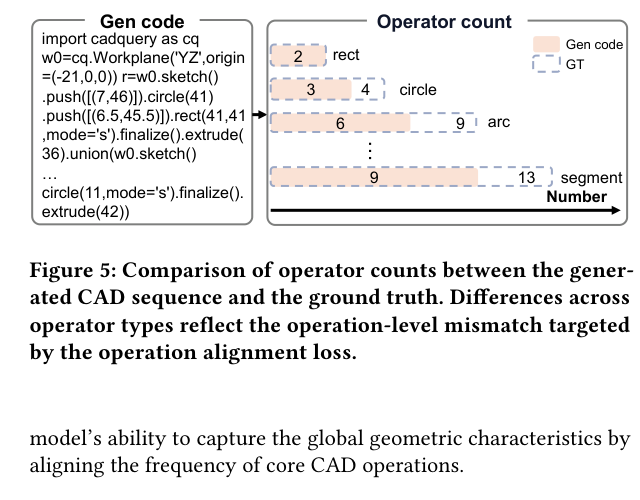
\includegraphics[width=\linewidth]{figures/operator_count.png}
\column{0.45\textwidth}
\small
\begin{align*}
\mathcal L_{\mathrm{SFT}}&=\mathcal L_{\mathrm{CE}}+\lambda_{\mathrm{SFT}}\mathcal L_{\mathrm{OP}},\\
\mathcal L_{\mathrm{CE}}&=-\frac1n\sum_{i=1}^n\log P(c_i\mid c_{<i},T_{\mathrm{pc}}).
\end{align*}
\begin{block}{动机}
漏掉一个 \texttt{circle} 或 \texttt{extrude}，可能导致整体几何出现明显错误。
\end{block}
\end{columns}
\source{原论文 Figure 5；式 (8), (10)，p.5}
\end{frame}

\begin{frame}{Stage 2 关键：可微的 Operation Soft Count}
\footnotesize
\begin{enumerate}\tight
\item GT 程序用字符串/模式匹配得到 $C_o^{\mathrm{GT}}$。
\item 生成程序的离散操作数通常不可微，改用预测概率之和：
\[
C_o^{\mathrm{pred}}=\sum_t p_t(o)\qquad\text{（单 Token 示意）}
\]
\item 实际运算需要枚举同一操作的多个 tokenization patterns，在每个序列位置求匹配概率，并在 log 空间聚合。
\item 原文给出操作对齐损失：
\[
\boxed{\mathcal L_{\mathrm{OP}}=1-\frac{1}{B}\sum_{b=1}^B
\mathrm{RIoU}(\bm C_b^{\mathrm{GT}},\bm C_b^{\mathrm{pred}})}
\]
\end{enumerate}
\begin{block}{解释边界}
操作\textbf{频次相同}不代表参数、位置、顺序或构造历史相同。
\end{block}
\source{原论文 §3.3.1，式 (9)，p.5；soft-count 简化式为教学推导}
\end{frame}

\begin{frame}{重要审查：操作计数的 RIoU 公式存在歧义}
\small
\tagunknown\ 原文把软分割掩码的 RIoU 形式应用于\textbf{可能大于 1 的计数向量}，但主文没有交代归一化。
\[
\mathrm{RIoU}(\bm a,\bm b)=\frac{\bm a^\top\bm b}{\lVert\bm a\rVert_1+\lVert\bm b\rVert_1-\bm a^\top\bm b}
\]
\begin{block}{直接代入原始 count 的反例}
$\bm a=(3,2),\ \bm b=(2,2)$，则内积为 $10$，两项 $L_1$ 范数之和为 $9$：
\[
\mathrm{RIoU}(\bm a,\bm b)=\frac{10}{9-10}=-10.
\]
这不具备通常 IoU 的取值范围。即使 $\bm a=\bm b=(3,2)$，也无法得到 1。
\end{block}
\taginfer\ 可考虑计数向量 generalized Jaccard $\sum\min(a_i,b_i)/\sum\max(a_i,b_i)$，\textbf{但不能当成作者实际实现}。
\source{原论文式 (5)、(9)；此页为独立的数学一致性检查}
\end{frame}

\begin{frame}{Stage 3：RL 让程序执行结果提供反馈}
\small
\begin{enumerate}\setlength{\itemsep}{0.55em}
\item 一个点云输入，采样 $K$ 个候选程序 $C_1,\ldots,C_K$。
\item 执行程序得到实体 $M(C_j)$；执行失败直接奖励 $-10$。
\item 成功实体与 GT 对齐、归一化，计算体积 IoU。
\item 从网格提取 Line / Arc / Circle，做 Feature-Line Matching。
\item 利用组内相对奖励进行 GRPO 策略更新。
\end{enumerate}
\begin{block}{奖励（原论文）}
\[
r=0.6\,\mathrm{IoU}(M^{\mathrm{GT}},M^{\mathrm{pred}})+0.4\,S_{\mathrm{feat}}(M^{\mathrm{GT}},M^{\mathrm{pred}}).
\]
\end{block}
\source{原论文 §3.4，式 (11)，pp.5–6}
\end{frame}

\begin{frame}{Stage 3：为什么小孔需要 Feature-Line Reward？}
\begin{columns}[c]
\column{0.49\textwidth}
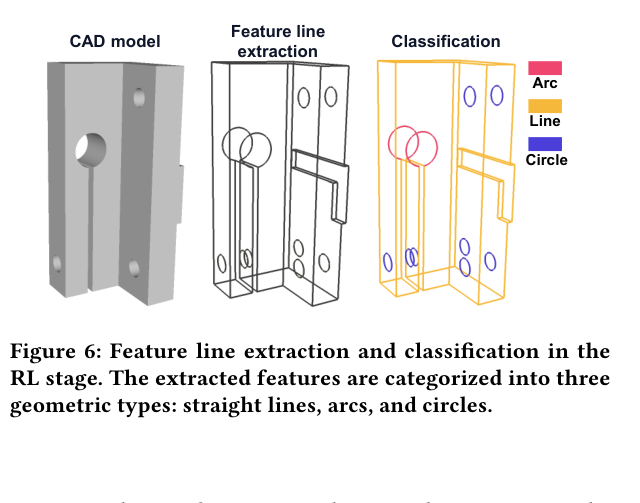
\includegraphics[width=\linewidth]{figures/feature_lines.png}
\column{0.5\textwidth}
\small
\begin{itemize}\setlength{\itemsep}{0.6em}
\item IoU 侧重重合体积；小孔体积占比低，遗漏时全局分数仍可能很高。
\item 特征线按 Line / Arc / Circle 分类。
\item 比较端点、中心偏移、长度比例、方向一致性等属性。
\item Hungarian Matching 最优配对，未匹配特征记零分。
\end{itemize}
\end{columns}
\source{原论文 Figure 6，pp.5–6；特征提取详细实现见论文 Supplementary}
\end{frame}

\begin{frame}{GRPO 的直觉：同组候选相互比较}
\small
给定同一个点云，得到多个候选程序与奖励：$r_1,\ldots,r_K$。
\[
\bar r=\frac1K\sum_{j=1}^K r_j,\qquad
\sigma_r=\sqrt{\frac1K\sum_{j=1}^K(r_j-\bar r)^2},\qquad
A_j\approx\frac{r_j-\bar r}{\sigma_r+\epsilon}.
\]
\begin{itemize}\setlength{\itemsep}{0.55em}
\item 高于组平均奖励的程序：正优势，倾向于提高其概率。
\item 低于组平均奖励的程序：负优势，倾向于降低其概率。
\item 不需要单独的价值网络，利用组内相对质量信号。
\end{itemize}
\begin{block}{注意}
这是 GRPO 的标准组相对优势直觉。PrimitiveCAD 正文未完整公开 clip / KL 等所有优化超参数。
\end{block}
\source{原论文 §3.4；GRPO 背景：DeepSeekMath, arXiv:2402.03300}
\end{frame}

\begin{frame}{推理时真正运行的 Pipeline}
\centering
\begin{tikzpicture}[node distance=0.7cm, every node/.style={font=\small}, block/.style={draw=teal,rounded corners,fill=light,minimum width=2.5cm,minimum height=1.15cm,align=center},arr/.style={-{Latex[length=2.8mm]},thick,draw=teal}]
\node[block] (p) {输入点云\\$P$};
\node[block,right=of p] (pt) {已训练的 PTv3\\FPS + Fourier};
\node[block,right=of pt] (t) {256 个\\连续几何 Tokens};
\node[block,right=of t] (llm) {已训练的 LLM\\CadQuery Python};
\draw[arr] (p)--(pt);\draw[arr] (pt)--(t);\draw[arr] (t)--(llm);
\node[block,below=0.95cm of llm] (cad) {执行 Python\\生成 CAD 实体};
\draw[arr] (llm)--(cad);
\end{tikzpicture}
\vspace{0.6em}
\begin{block}{与训练流程的区别}
推理不需要\textbf{GT Primitive 标签、GT CAD 程序、Operation Count Loss 或 RL Reward}。这些都用于训练模型参数。
\end{block}
\end{frame}

\section{实验}
\begin{frame}{6. 实验怎么设计：Claim $\to$ Experiment $\to$ Answer}
\small
\begin{table}\centering
\begin{tabular}{p{3.75cm}p{4.75cm}p{3.5cm}}\toprule
研究问题 & 验证实验 & 论文结论\\\midrule
整体方法更好吗？ & DeepCAD、Fusion360；IoU/CD/IR & 整体性能提升\\
CAD PTv3 监督有用吗？ & 去掉 PTv3 finetuning & 有，IoU 降低\\
Operator Alignment 有用吗？ & 去掉 $\mathcal L_{\mathrm{OP}}$ & 有，IoU 降低\\
特征线奖励有用吗？ & RL 有/无 $S_{\mathrm{feat}}$ & 增量改善，尤其最差样本\\
RL 稳定输出吗？ & 10 次采样的 best/worst & worst 结果明显改善\\
点越多越好吗？ & 512/1024/2048/4096 点 & 1024 是较好折中\\\bottomrule
\end{tabular}
\end{table}
\source{原论文 §4，Tables 1–5，pp.6–8}
\end{frame}

\begin{frame}{主要结果：同样 DCAD+CADR 训练配置的比较}
\small
\begin{table}\centering
\begin{tabular}{lccc}\toprule
方法（SFT，无 RL） & DeepCAD IoU $\uparrow$ & Fusion360 IoU $\uparrow$ & Fusion360 IR $\downarrow$\\\midrule
Cadrille & 86.6 & 76.5 & 2.0\\
\textbf{PrimitiveCAD} & \textbf{90.9} & \textbf{84.9} & \textbf{0.4}\\\bottomrule
\end{tabular}
\end{table}
\begin{block}{直接结论}
在论文的对比条件下，Fusion360 IoU 从 76.5 提升到 84.9（\textbf{+8.4 个百分点}）；IR 从 2.0 降至 0.4。
\end{block}
\begin{itemize}\tight
\item 指标：IoU 是体积交并比；IR 是无效 CAD 程序比例。
\item Table 1 是\textbf{无 RL、无 test-time sampling} 的对比。
\item 不同训练数据配置之间不能直接解释为同等控制变量实验。
\end{itemize}
\source{原论文 Table 1，p.7}
\end{frame}

\begin{frame}{消融 1：SFT 的两种结构监督确实贡献性能}
\begin{columns}[T]
\column{0.47\textwidth}
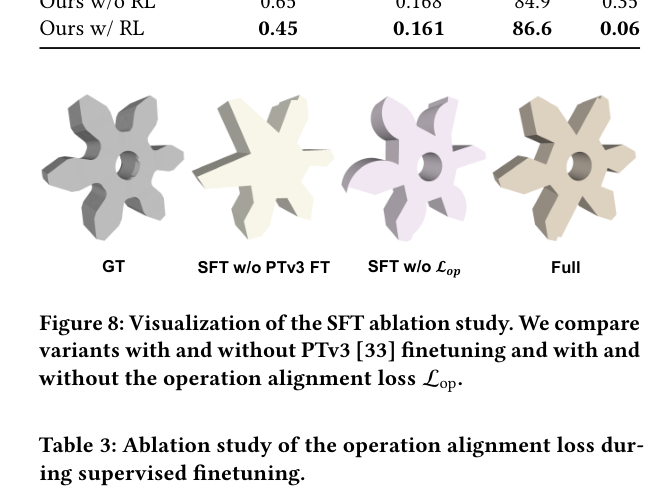
\includegraphics[width=\linewidth]{figures/sft_ablation.png}
\column{0.53\textwidth}
\small
\begin{table}\centering
\begin{tabular}{lrr}\toprule
Fusion360 & IoU$\uparrow$ & Mean CD$\downarrow$\\\midrule
无 PTv3 微调 & 82.4 & 0.88\\
无 OP Loss & 83.4 & 0.71\\
\textbf{完整 SFT} & \textbf{84.9} & \textbf{0.65}\\\bottomrule
\end{tabular}
\end{table}
\begin{block}{证据边界}
有效性体现在几何 IoU/CD；还不能单靠这张表证明 OP Loss 一定降低\textbf{真实操作计数错误率}。
\end{block}
\end{columns}
\source{原论文 Figure 8 / Table 3，p.8}
\end{frame}

\begin{frame}{消融 2：RL 主要改善较差采样结果}
\begin{columns}[T]
\column{0.48\textwidth}
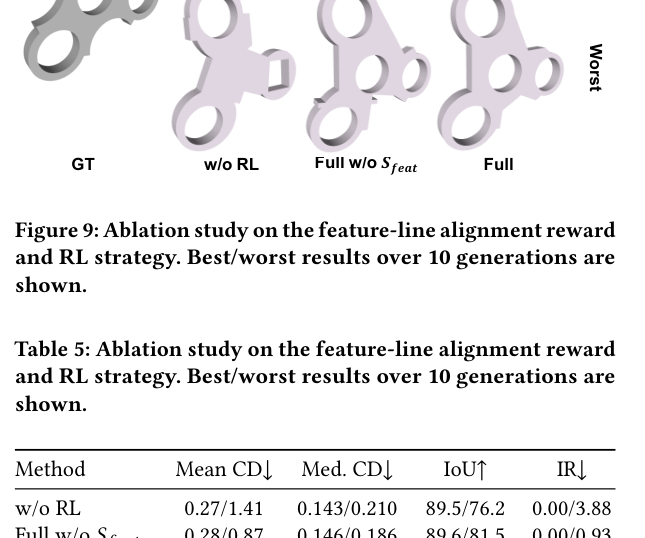
\includegraphics[width=\linewidth]{figures/rl_ablation.png}
\column{0.52\textwidth}
\small
\begin{table}\centering
\begin{tabular}{lrr}\toprule
方法 & Best IoU & Worst IoU\\\midrule
无 RL & 89.5 & 76.2\\
RL 无特征奖励 & 89.6 & 81.5\\
\textbf{完整 RL} & \textbf{89.6} & \textbf{82.3}\\\bottomrule
\end{tabular}
\end{table}
\taginfer\ 无 RL $\to$ RL：worst IoU +5.3；加入 Feature Reward 再提升 +0.8。\textbf{主要稳定性收益来自 RL 本身}。
\end{columns}
\source{原论文 Figure 9 / Table 5，p.8；best/worst 为 10 次采样结果}
\end{frame}

\begin{frame}{SFT 与 RL：最值得记住的一组对照}
\small
\begin{table}\centering
\begin{tabular}{lrrrr}\toprule
Fusion360 & Mean CD$\downarrow$ & Median CD$\downarrow$ & IoU$\uparrow$ & IR$\downarrow$\\\midrule
Cadrille SFT & 1.05 & 0.220 & 76.5 & 2.00\\
Cadrille RL & 0.58 & 0.176 & 84.8 & 0.46\\
\textbf{PrimitiveCAD SFT} & 0.65 & 0.168 & \textbf{84.9} & 0.35\\
\textbf{PrimitiveCAD RL} & \textbf{0.45} & \textbf{0.161} & \textbf{86.6} & \textbf{0.06}\\\bottomrule
\end{tabular}
\end{table}
\begin{block}{核心观察}
\textbf{PrimitiveCAD 只做 SFT（84.9 IoU）}，就接近/略高于 Cadrille 的 RL 版本（84.8）。这支持先改善输入表示和 SFT 目标再增加 RL 的研究路线。
\end{block}
\source{原论文 Table 2，p.8}
\end{frame}

\begin{frame}{定性结果：孔、直角和复杂局部结构}
\centering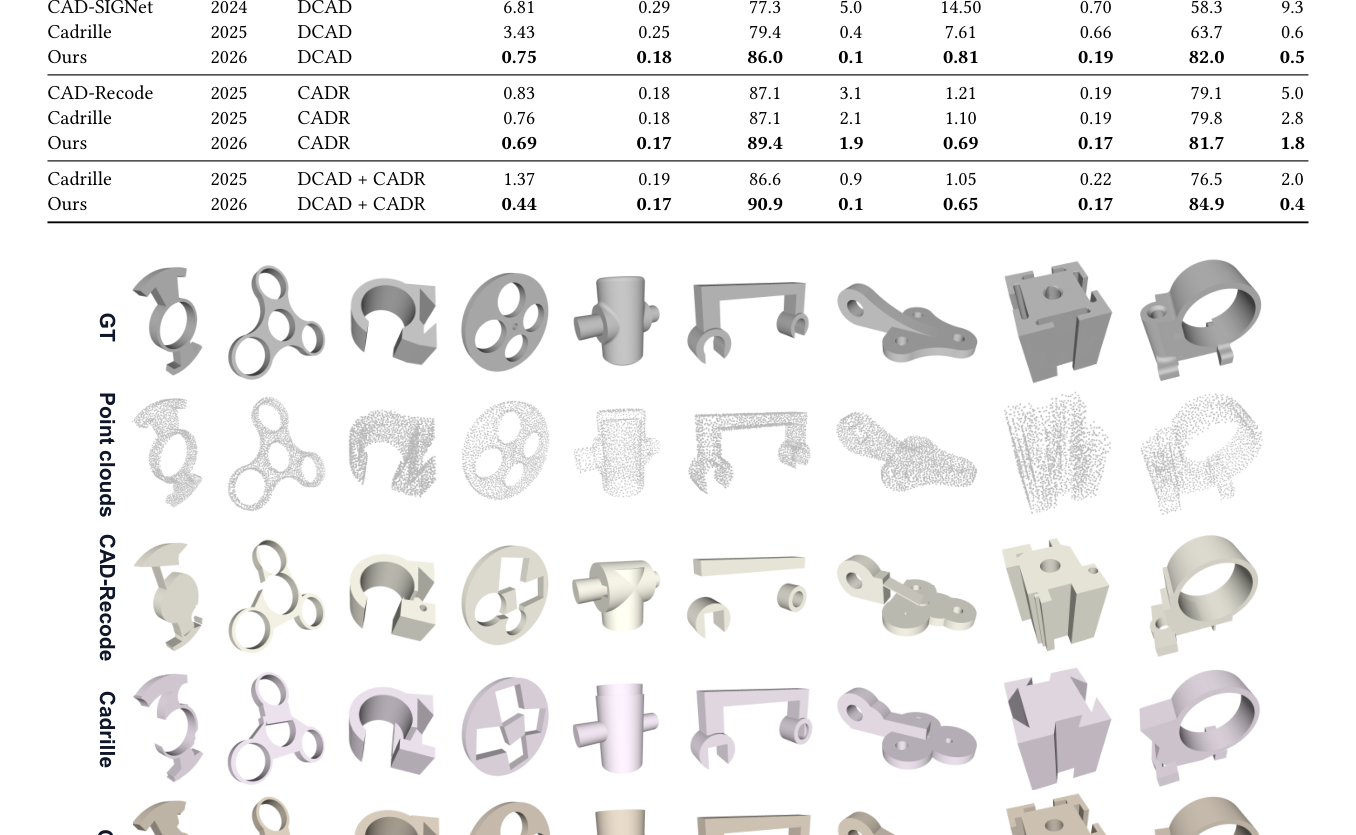
\includegraphics[width=0.98\linewidth,height=0.75\textheight,keepaspectratio]{figures/qualitative.png}
\source{原论文 Figure 7，p.7；\textbf{定性图为每个方法 10 个候选中的最佳结果}，与 Table 1 的单次采样评价不同}
\end{frame}

\begin{frame}{实验的三个未闭合问题}
\begin{enumerate}\setlength{\itemsep}{0.95em}
\item \textbf{缺少直接证明机制的指标。} IoU 提升不等价于 Operator Count MAE 下降或 Hole Recall 提升。
\item \textbf{缺少充分的真实扫描域外证据。} 噪声、遮挡、非均匀采样和稀疏小孔是否鲁棒，正文没有系统量化。
\item \textbf{缺少设计意图/编辑性的测量。} 可执行程序与参数化建模质量不是同义词；还需要编辑成功率与约束保持率。
\end{enumerate}
\begin{block}{同样需要核对的实现}
Operation RIoU 的归一化；面重叠时的 Primitive Label；网格域 Feature-Line Extraction；奖励特征尺度归一化。
\end{block}
\end{frame}

\section{批判与未来研究}
\begin{frame}{7. Takeaways 与最脆弱的假设}
\small
\begin{columns}[T]
\column{0.5\textwidth}
\begin{block}{Takeaways}
\begin{enumerate}\tight
\item 通用点云特征不一定最适合 CAD。
\item 结构化代码需要超越逐 Token 的训练信号。
\item 评价函数应对工程重要的小特征敏感。
\item 强化 SFT 可能减少对昂贵 RL 的依赖。
\end{enumerate}
\end{block}
\column{0.48\textwidth}
\begin{block}{脆弱假设}
\begin{enumerate}\tight
\item 四类 Primitive + 32 槽位是否足够？
\item 操作频次是否足以约束构造语义？
\item 几何相似是否代表\textbf{可编辑、可制造}的设计？
\end{enumerate}
\end{block}
\end{columns}
\vspace{0.65em}
\centering
$\bm C_A=\bm C_B\;\not\Rightarrow\;M(C_A)=M(C_B)$\\[0.3em]
\small 同操作次数的程序，孔位置、尺寸和拓扑仍可能不同。
\end{frame}

\begin{frame}{8. 一周最小复现：专测 Operation Alignment}
\small
\begin{table}\centering
\begin{tabular}{lp{10.3cm}}\toprule
时间 & 工作\\\midrule
Day 1 & CadQuery 合成几千个板/孔/拉伸程序；保存 GT 代码与操作向量\\
Day 2 & 检查原文 RIoU 定义；实现 Soft Count 与合理的计数损失基线\\
Day 3–4 & 固定输入编码器，控制参数与训练步骤；比较 CE-only 和 CE+Count\\
Day 5 & 构造同次数不同孔位、更多孔、不同构造方式的分布外测试\\
Day 6–7 & 分析计数误差、几何 IoU、IR 和失败类型\\\bottomrule
\end{tabular}
\end{table}
\begin{block}{最关键的指标}
Operator Count MAE / Exact Count Accuracy / Geometry IoU / Invalidity Rate。
\end{block}
\taginfer\ 计数更准但 IoU 不提高，将直接揭示全局统计监督的边界。
\end{frame}

\begin{frame}{9. 如何反对它：三个可证伪反例}
\small
\begin{enumerate}\setlength{\itemsep}{0.95em}
\item \textbf{同操作次数，不同几何：} 构造三孔板，保持 circle 数量不变，仅改变孔中心。测试 Operation Loss 是否真的改善参数与空间配置。
\item \textbf{同几何，低编辑质量：}两个程序当前 IoU 都接近 1，修改板宽后检查孔径、孔距和对称约束是否保持。
\item \textbf{小孔没有被观察到：}减小孔面积和点云密度，制造孔壁采样为零或近零的输入。检验模型的可观测性边界。
\end{enumerate}
\begin{block}{重要区分}
第 1 项检验\textbf{监督信息不足}；第 2 项检验\textbf{评价目标偏差}；第 3 项检验\textbf{输入信息不可辨识}。
\end{block}
\end{frame}

\begin{frame}{10. Follow-up：从几何重建转向设计意图恢复}
\begin{block}{Equivalence-Aware CAD Reconstruction with Executable Design Constraints}
\textbf{新问题：}不只输出几何近似的程序，还要让程序在参数编辑之后保持可验证的设计约束。
\end{block}
\small
\[
\max_C\quad R_{\mathrm{geometry}}(C)
+\lambda R_{\mathrm{edit}}(C)
+\mu R_{\mathrm{constraint}}(C)
-\nu R_{\mathrm{complexity}}(C).
\]
\begin{itemize}\tight
\item \textbf{Geometry：}静态实体的形状误差。
\item \textbf{Edit：}修改宽度/孔径等参数后是否正确响应。
\item \textbf{Constraint：}对称、同心、等径、平行关系是否仍然成立。
\item \textbf{Complexity：}避免冗长且脆弱的构造代码。
\end{itemize}
\tagunknown\ 这是基于论文缺陷提出的研究假设，\textbf{不是 PrimitiveCAD 已验证的结果}。
\end{frame}

\begin{frame}{Follow-up 的最小研究设计}
\small
\begin{columns}[T]
\column{0.5\textwidth}
\begin{block}{数据构造}
\begin{enumerate}\tight
\item 编写含参数约束的 CAD 生成程序。
\item 随机实例化参数，生成实体与点云。
\item 采样参数编辑任务并重新执行程序。
\item 验证编辑后几何与设计约束。
\end{enumerate}
\end{block}
\column{0.47\textwidth}
\begin{block}{Benchmark}
\begin{itemize}\tight
\item Edit Success Rate
\item Constraint Preservation Rate
\item Edit-induced Geometry Error
\item Original Geometry IoU
\item Program Complexity
\end{itemize}
\end{block}
\end{columns}
\vspace{0.5em}
\begin{block}{挑战}
仅凭一个静态点云通常无法唯一识别原作者的建模意图；应允许\textbf{多个候选解释}或引入额外的设计要求。
\end{block}
\end{frame}

\begin{frame}{结论：读完 PrimitiveCAD 需要记住什么？}
\begin{enumerate}\setlength{\itemsep}{0.95em}
\item \textbf{研究路线清晰：}在表示、代码生成和几何反馈三个层面加入 CAD 专用结构信息。
\item \textbf{实验支持提升：}在主要公开测试集上，SFT 和完整 RL 都改善几何准确性与程序有效性。
\item \textbf{机制需要更直接证据：}特别是操作数量误差、局部孔/线指标以及真实扫描鲁棒性。
\item \textbf{最大后续空间：}从 static geometry accuracy 推进到 editable CAD + design constraints。
\end{enumerate}
\begin{block}{一句话}
把 CAD 当作\textbf{结构化、可执行、可编辑的几何程序}，才能进一步突破静态形状相似度评价的局限。
\end{block}
\end{frame}

\begin{frame}{参考文献与材料说明}
\footnotesize
\begin{enumerate}\setlength{\itemsep}{0.43em}
\item Gao et al. \textit{PrimitiveCAD: An LLM-Based Point-to-CAD Reconstruction with Primitive-Aware Tokenization and Operation Alignment}. ACM MM 2026. \url{https://arxiv.org/abs/2610.08698}
\item Rukhovich et al. \textit{CAD-Recode: Reverse Engineering CAD Code from Point Clouds}. ICCV 2025.
\item Kolodiazhnyi et al. \textit{Cadrille: Multi-modal CAD Reconstruction with Reinforcement Learning}. 2025.
\item Wu et al. \textit{Point Transformer V3: Simpler, Faster, Stronger}. CVPR 2024.
\item Wu et al. \textit{DeepCAD: A Deep Generative Network for Computer-Aided Design Models}. ICCV 2021.
\item Shao et al. \textit{DeepSeekMath: Pushing the Limits of Mathematical Reasoning in Open Language Models}. 2024.
\end{enumerate}
\vspace{0.5em}
\textbf{图片版权/来源：} Figures 1–9 的裁剪图均出自上传的 PrimitiveCAD 论文。正文标示 CC BY 4.0，保留来源说明。\\[0.3em]
\textbf{编译环境：}Overleaf $\rightarrow$ XeLaTeX，主文件 \texttt{main.tex}，所有图片位于 \texttt{figures/}。
\end{frame}

\end{document}